\PassOptionsToPackage{unicode=true}{hyperref} % options for packages loaded elsewhere
\PassOptionsToPackage{hyphens}{url}
%
\documentclass[]{article}
\usepackage{lmodern}
\usepackage{amssymb,amsmath}
\usepackage{ifxetex,ifluatex}
\usepackage{fixltx2e} % provides \textsubscript
\ifnum 0\ifxetex 1\fi\ifluatex 1\fi=0 % if pdftex
  \usepackage[T1]{fontenc}
  \usepackage[utf8]{inputenc}
  \usepackage{textcomp} % provides euro and other symbols
\else % if luatex or xelatex
  \usepackage{unicode-math}
  \defaultfontfeatures{Ligatures=TeX,Scale=MatchLowercase}
\fi
% use upquote if available, for straight quotes in verbatim environments
\IfFileExists{upquote.sty}{\usepackage{upquote}}{}
% use microtype if available
\IfFileExists{microtype.sty}{%
\usepackage[]{microtype}
\UseMicrotypeSet[protrusion]{basicmath} % disable protrusion for tt fonts
}{}
\IfFileExists{parskip.sty}{%
\usepackage{parskip}
}{% else
\setlength{\parindent}{0pt}
\setlength{\parskip}{6pt plus 2pt minus 1pt}
}
\usepackage{hyperref}
\hypersetup{
            pdftitle={Web Tool for Basic Plotting and Analysis},
            pdfauthor={Foo Cheung},
            pdfborder={0 0 0},
            breaklinks=true}
\urlstyle{same}  % don't use monospace font for urls
\usepackage[margin=1in]{geometry}
\usepackage{graphicx,grffile}
\makeatletter
\def\maxwidth{\ifdim\Gin@nat@width>\linewidth\linewidth\else\Gin@nat@width\fi}
\def\maxheight{\ifdim\Gin@nat@height>\textheight\textheight\else\Gin@nat@height\fi}
\makeatother
% Scale images if necessary, so that they will not overflow the page
% margins by default, and it is still possible to overwrite the defaults
% using explicit options in \includegraphics[width, height, ...]{}
\setkeys{Gin}{width=\maxwidth,height=\maxheight,keepaspectratio}
\setlength{\emergencystretch}{3em}  % prevent overfull lines
\providecommand{\tightlist}{%
  \setlength{\itemsep}{0pt}\setlength{\parskip}{0pt}}
\setcounter{secnumdepth}{5}
% Redefines (sub)paragraphs to behave more like sections
\ifx\paragraph\undefined\else
\let\oldparagraph\paragraph
\renewcommand{\paragraph}[1]{\oldparagraph{#1}\mbox{}}
\fi
\ifx\subparagraph\undefined\else
\let\oldsubparagraph\subparagraph
\renewcommand{\subparagraph}[1]{\oldsubparagraph{#1}\mbox{}}
\fi

% set default figure placement to htbp
\makeatletter
\def\fps@figure{htbp}
\makeatother


\title{Web Tool for Basic Plotting and Analysis}
\author{Foo Cheung}
\date{2021-05-25}

\begin{document}
\maketitle

\newpage 
\tableofcontents 
\newpage

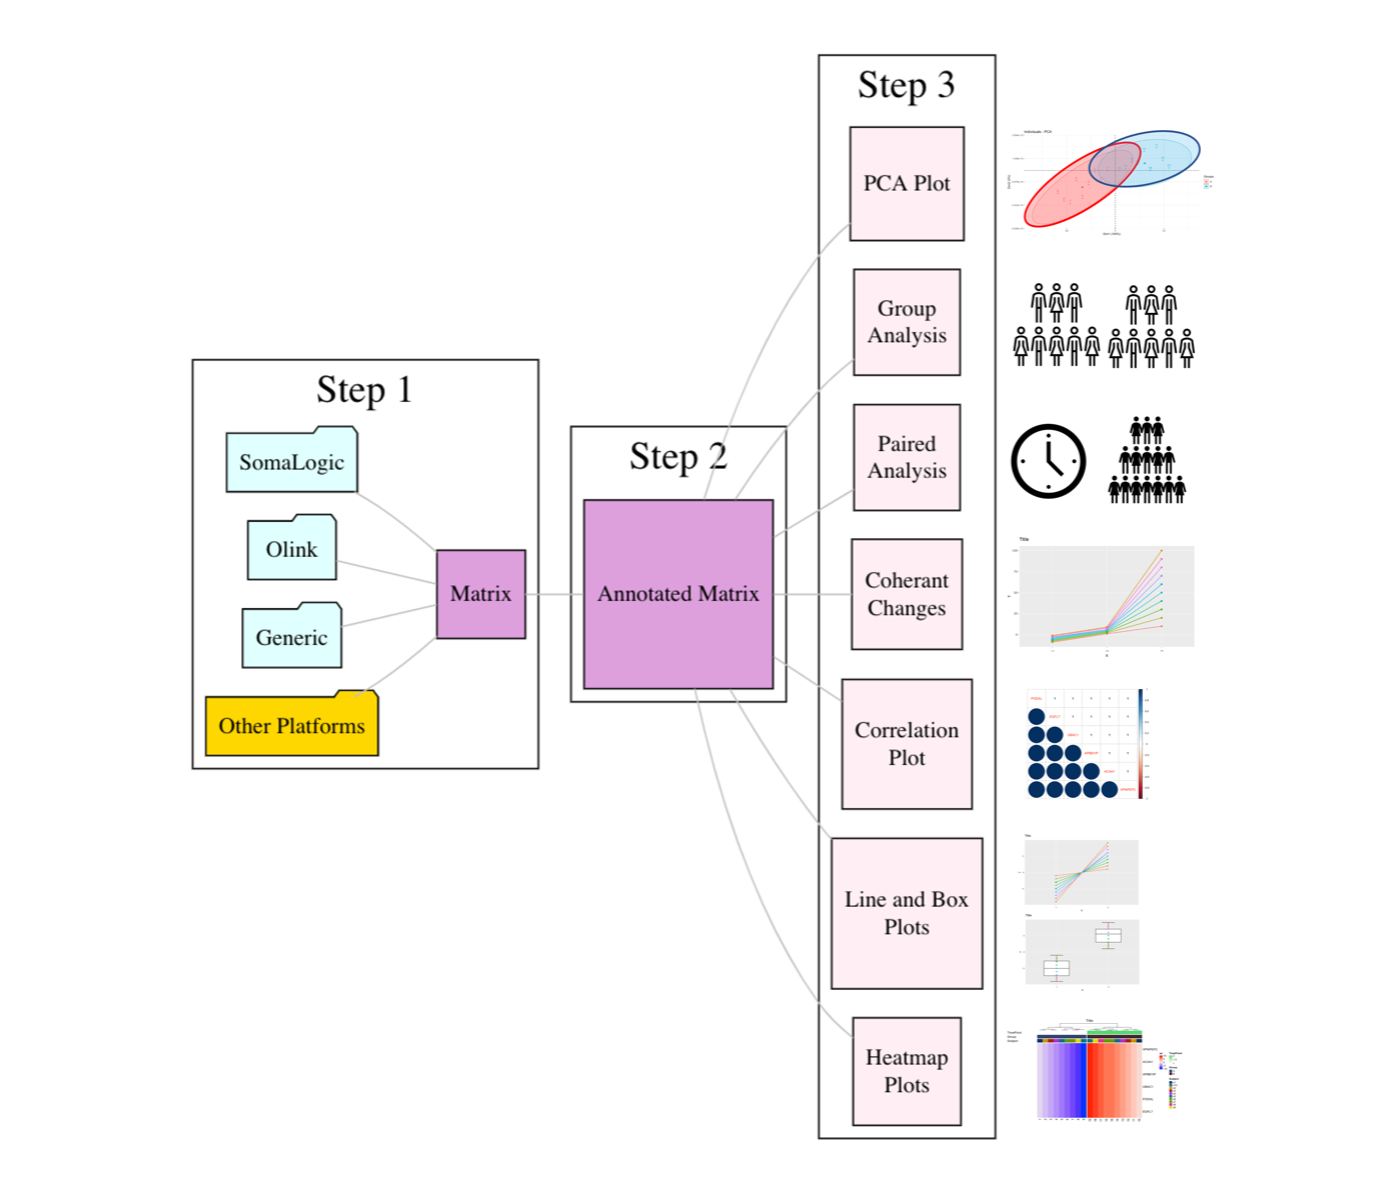
\includegraphics[width=0.8\textwidth,height=\textheight]{./overview_pipeline.png}

\hypertarget{overview}{%
\subsection{Overview}\label{overview}}

This Web Tool was designed to be a user- friendly tool for the
``non-bioinformaticians'' to do preliminary analyses of proteomic
(SomaLogic and Olink) and other data sets. The most up-to-date version
of the tool can be accessed here: Below you will find some pointers for
using the tool.

In addition to specific tool instructions, this document includes some
suggestions for analyses. Please note that these are simply guidelines
found to be useful based on previous experience. Every project is unique
and these guidelines should be adapted as necessary.

For further, please reach out to Foo Cheung at
\href{mailto:foo.cheung@nih.gov}{\nolinkurl{foo.cheung@nih.gov}}.

\newpage

\hypertarget{quick-start-guide}{%
\subsection{Quick Start Guide}\label{quick-start-guide}}

\textbf{As Easy As Step 1, 2 And 3}

This section demonstrates how to prepare and analyze data.

\textbf{Step 1.} Select the correct entry page revelvant to your
dataset:

\begin{itemize}
\tightlist
\item
  SomaLogic
\item
  Olink
\item
  Generic
\end{itemize}

Step 1 entails converting your proteomic (e.g., SomaLogic or Olink) or
other data from any source into a tab-delimited text file that contains
a column for each sample, a row for each gene, and an expression value
for each target in each sample. Upload your data file as Input for
matrix conversion, then download the resulting output file. Annotate the
SampleID, Subject, Group and TimePoint columns. Save the file as a tab
delimited text file, ready for uploading at Step2.

\textbf{Step 2.} Step 2 entails uploading your manually annotated file
from Step 1, use the available features to filter the samples (rows) and
assay data (columns) and proceed to Step3

\textbf{Step 3.} Use The Available Tools For Basic Analysis and Plotting
Step 3 entails selecting the available tools to analyze and plot your
data

\newpage

\hypertarget{user-manual}{%
\section{User Manual}\label{user-manual}}

\hypertarget{step-1}{%
\subsection{Step 1}\label{step-1}}

Step 1 entails converting your proteomic (e.g., SomaLogic or Olink) or
other data from any source into a tab-delimited text file that contains
a column for each sample, a row for each gene, and an expression value
for each target in each sample.

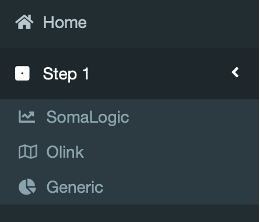
\includegraphics[width=0.3\textwidth,height=\textheight]{./step1.png}

 Click on the tab ``Step 1'', you will be offered links to process
different data sets. Click on the appropriate link for you data.

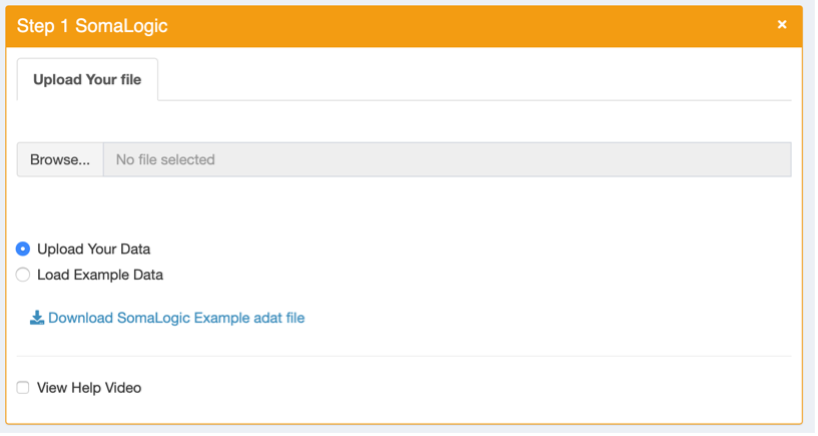
\includegraphics[width=0.5\textwidth,height=\textheight]{./step1_1.png}

 For Example: clicking on ``SomaLogic'' will bring up the box shown
above.

Either upload your adat data file by clicking on ``Browse'' or ``Load
Example Data'' to explore the features of the app without uploading any
data.

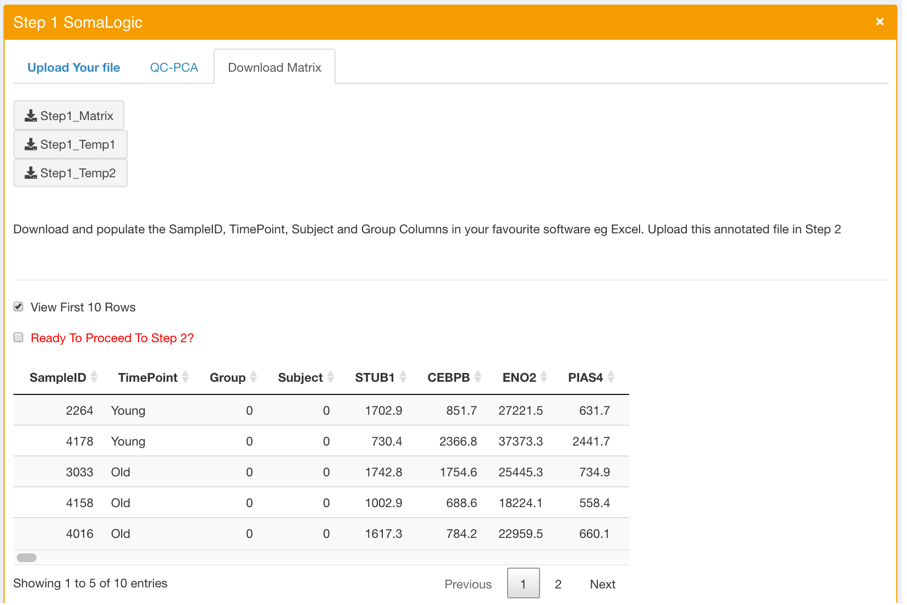
\includegraphics[width=0.5\textwidth,height=\textheight]{./step1_2.png}

 Click on the ``Step1\_Matrix'' button and annotate the SampleID
(unique), TimePoint, Group and Subject column before Proceeding to Step
2 by clicking on the ``Go To Step 2'' button.

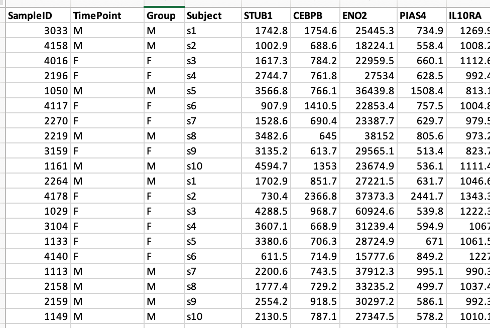
\includegraphics[width=0.5\textwidth,height=\textheight]{./step1_3.png}

 Before moving on different tabs you can also perform a Principal
component analysis (PCA) on the data by clicking on the QC-PCA tab. The
Samples, Buffers, Controls are plotted as a scatterplot along the top 2
principal components. These plots can provide useful QC checks by
showing clusters based on SampleType for example: Buffers versus Samples
versus controls or checking if different plates show a batch effect.

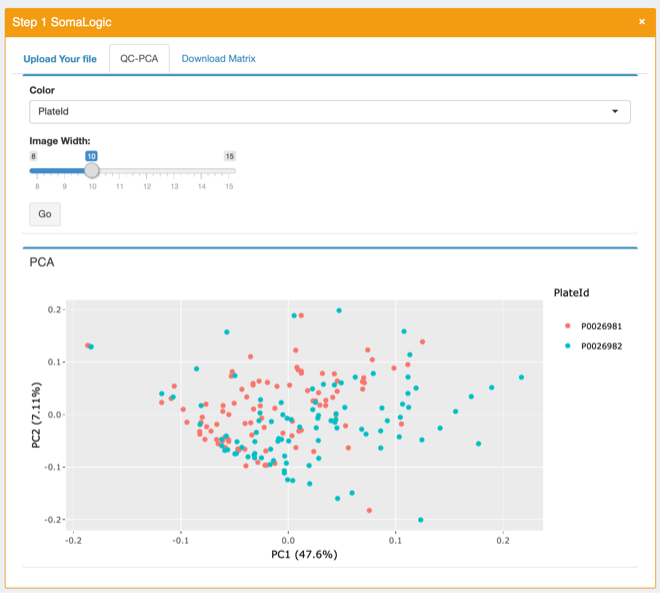
\includegraphics[width=0.5\textwidth,height=\textheight]{./step1_4.png}

\newpage

\hypertarget{step-2}{%
\subsection{Step 2}\label{step-2}}

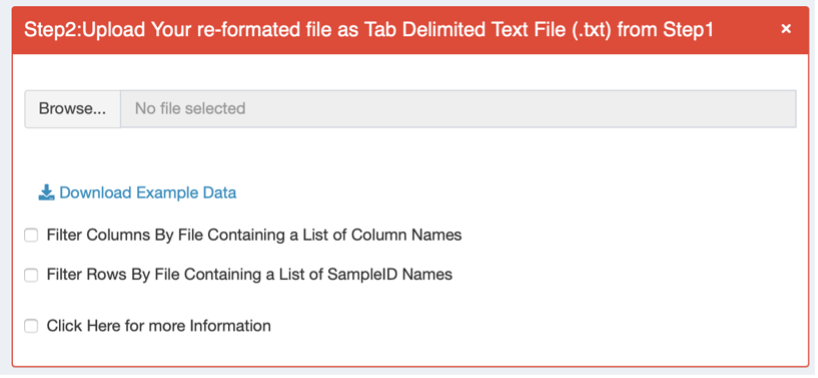
\includegraphics[width=0.5\textwidth,height=\textheight]{./step2.png}

 \textbf{File Format:} The current tool requires you upload your file as
a \textbf{Tab Delimted text file (.txt)}. You can make modifications to
the data file in Excel for example, but be sure to export the file to a
\textbf{tab delimited format}.

Prior to uploading data, it is \textbf{important} to make sure
\textbf{SampleID, TimePoint, Subject and Group columns}, as well as any
other columns intended for use during the analysis, were annotated
consistently.

Click on the ``Browse'' button and upload your annotated Tabbed
Delimited Text data file (that you download \textbf{from Step 1} and
then annotated for \textbf{SampleID (must be unique)}, TimePoint, Group
and Subject column). \textbf{If there are no TimePoint and/or Group
information, please enter 0 and do not leave them blank or NA}. The
SampleID must be unique and containing no NA or blank values. \textbf{If
there is only one Sample per Subject then the SampleID can be safely
copied over to the Subject column}.

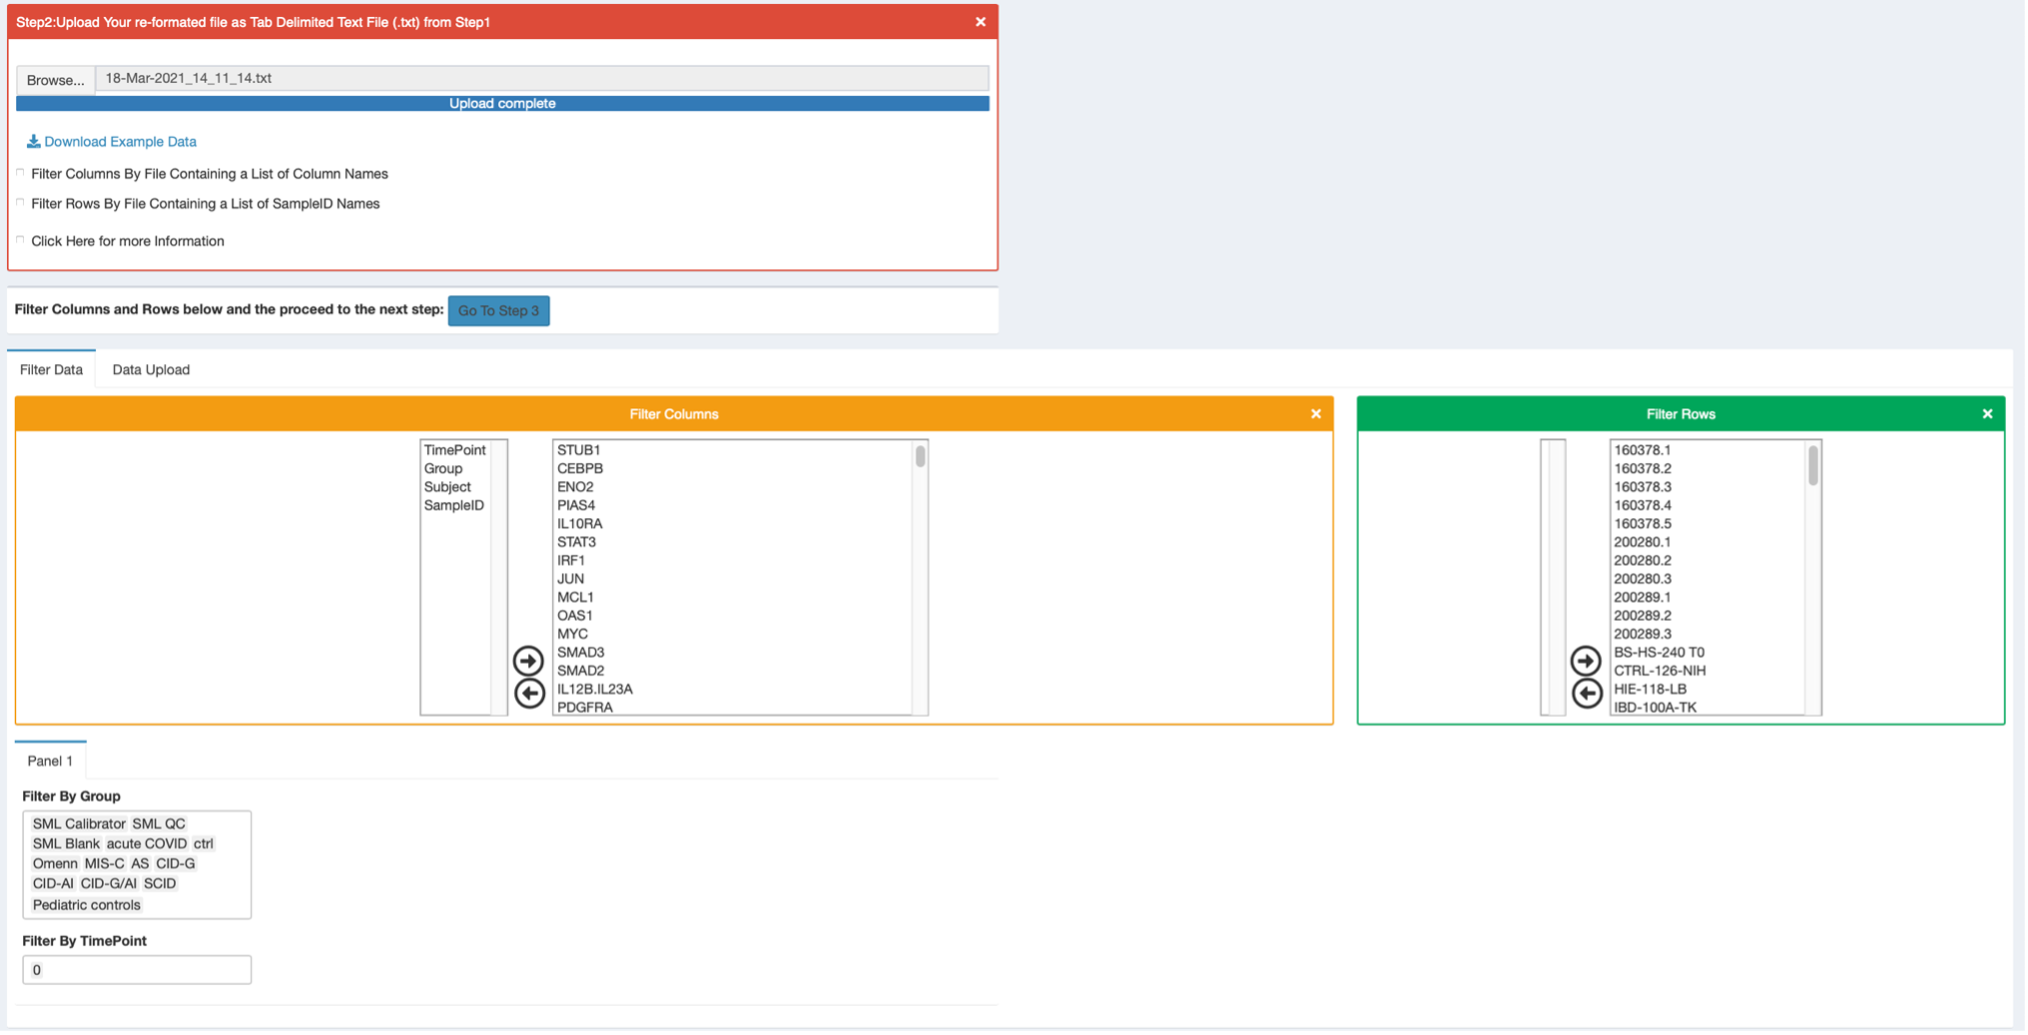
\includegraphics[width=0.7\textwidth,height=\textheight]{step2_2.png}

\textbf{Filtering both Samples (rows) and analytes (columns) can be done
in a number of ways as shown below:}

\begin{enumerate}
\def\labelenumi{\arabic{enumi}.}
\tightlist
\item
  Upload a single column of Samples or/and analytes that can filter out
  data automatically
\item
  Manually filter rows/samples or/and analytes/columns using the dual
  list box shown above
\item
  Filter Samples by using the annotated Group and or TimePoint
  information attached to each Sample
\end{enumerate}

\newpage

\hypertarget{step-3}{%
\subsection{Step 3}\label{step-3}}

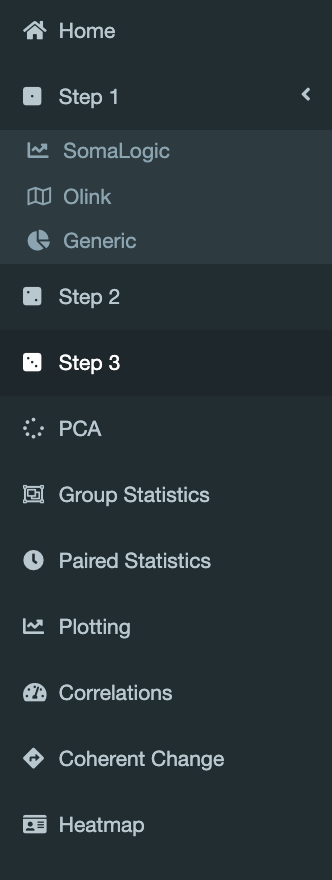
\includegraphics[width=0.2\textwidth,height=\textheight]{./step3.png}

Clicking on the Step 3 button should allow the user to perform various
analysis and plots as above.

\newpage

\hypertarget{pca}{%
\subsubsection{PCA}\label{pca}}

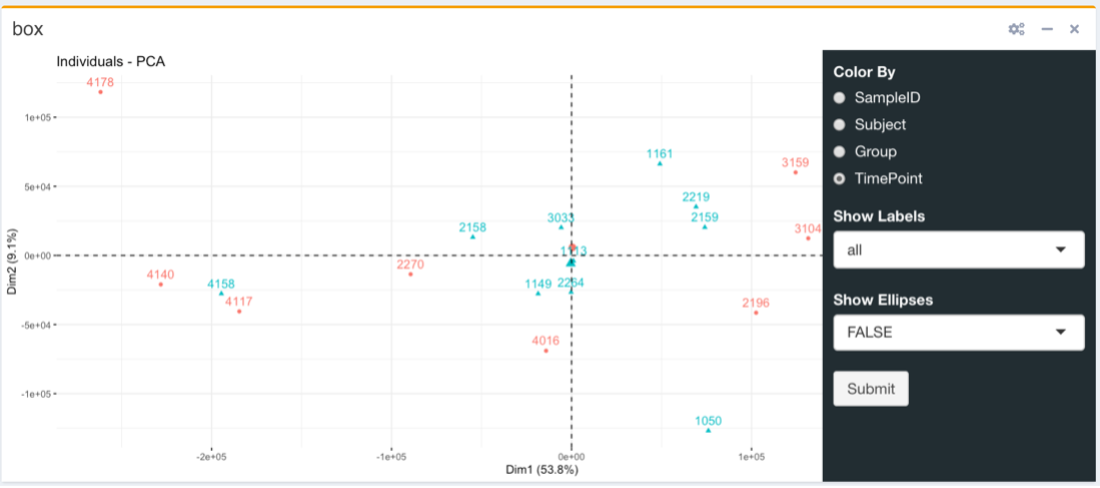
\includegraphics[width=0.5\textwidth,height=\textheight]{./step3_1.png}

The Principle Component Analysis (PCA) is a tool used to reduce the
dimensionality of datasets to increase interpretability by creating new
uncorrelated variables that successively maximize variance. Principal
Component Analysis (PCA) is a technique used to emphasize variation and
bring out strong patterns in a dataset (dimensionality reduction).
Various options to color by different variables and show or hide labels
is made available to the user by way of the menu.

\newpage

\hypertarget{group-statistics}{%
\subsubsection{Group Statistics}\label{group-statistics}}

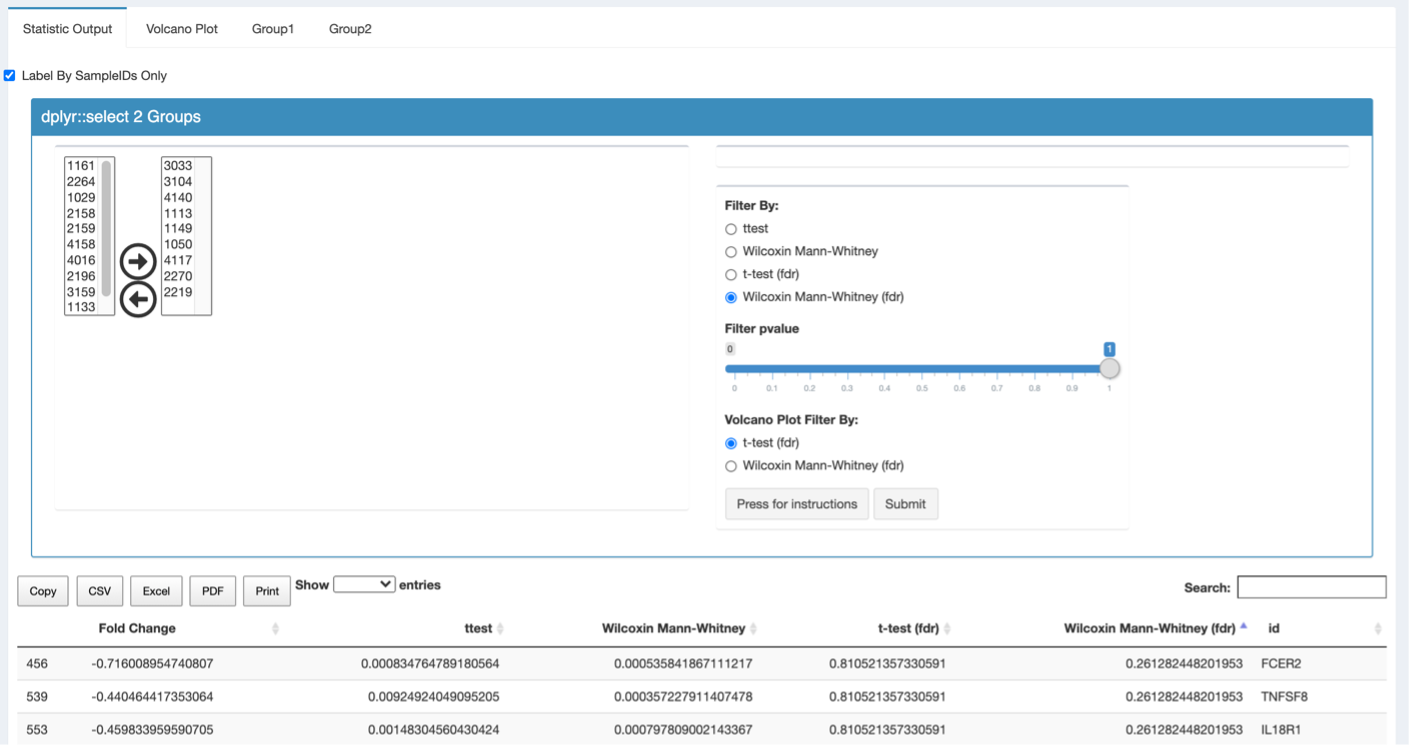
\includegraphics[width=0.7\textwidth,height=\textheight]{./step3_2.png}

If you ran an experiment comparing two or more separate patient groups,
such as diseased and healthy, you should use this Group Statistics
option. Please note that this tool only allows you to compare two groups
at a time. If you ran an experiment comparing one set of patients at
multiple time points, you should use the Paired Data tab. Post Analysis:
After you identify the most statistically significant results, as a
quick QC, it is recommended you utilize the BoxPlots tool and plot the
identified analyte and sample groups to visualize the difference.\\
This tool can append the SampleGroup and TimePoint to the SampleID,
separated by an underscore. The samples can then be separated into two
groups more easily based on the additional information attached to the
data. The most powerful results will be evident in the fdr corrected
data where the smallest value (the statistical p-value) is the most
significant. To sort the output by smallest to largest in a column,
select the gray arrows next to the statistical test name. If analyses
reveal only a few significant analytes in the fdr corrected data, then
reference the non-fdr corrected data. It is important to QC the groups
that were analyzed to make sure that the samples you expected to be in
the group(s), were in fact there. Results can be exported into various
file formats including PDF and excel. To export the full list of
results, be sure to update the Show \_\_ entries box to be Show nth
entries. If you do not make this change, the exported file will only
contain the list of results currently visible in the browser. Volcano
Plot, this tab will display a scatter plot of analytes statistical
significance versus fold-change. The plot will show transformed p-value
of the non-fdr corrected Wilcox Mann-Whitney. The plot does denote the
fdr-corrected significant analytes with color coding. Although not
called out, the Fold Change on the x-axis is a log2 scale.

\newpage

\hypertarget{paired-statistics}{%
\subsubsection{Paired Statistics}\label{paired-statistics}}

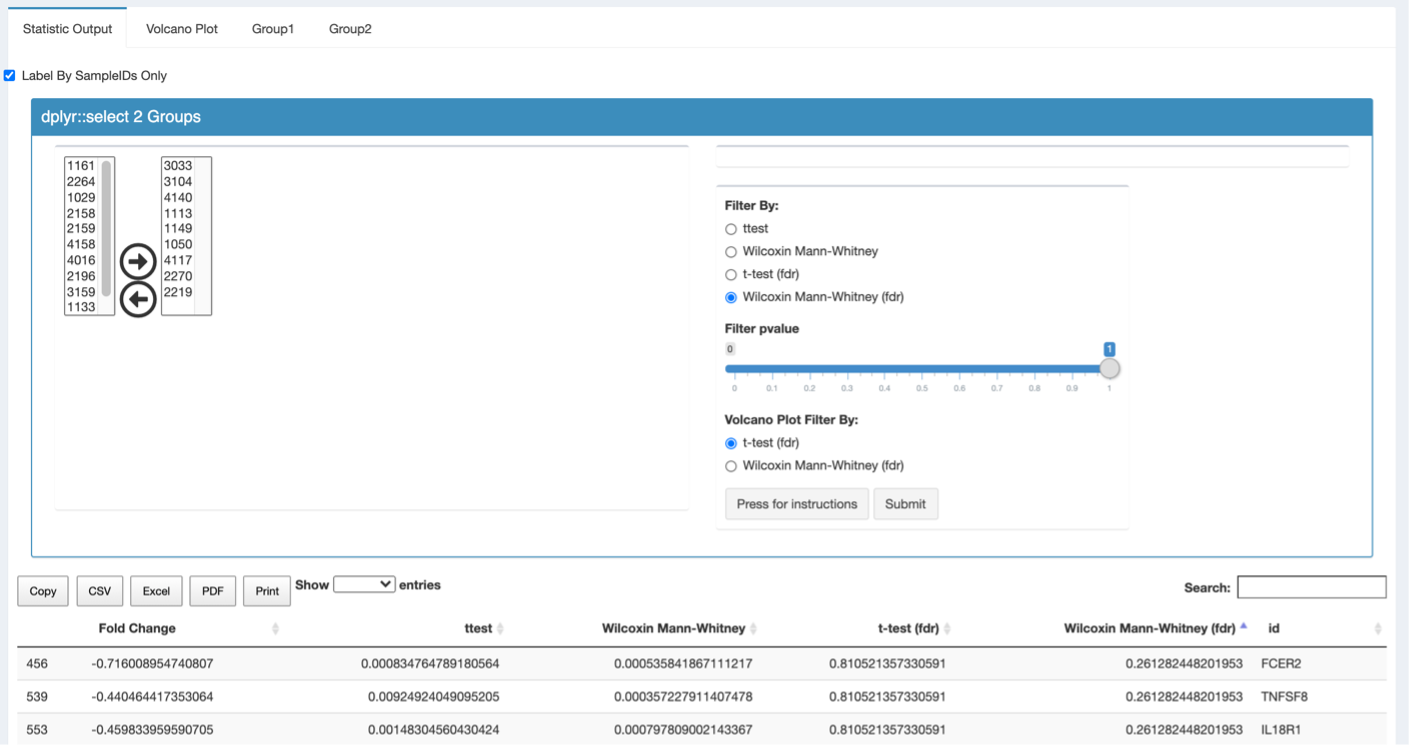
\includegraphics[width=0.7\textwidth,height=\textheight]{./step3_3.png}

A paired t-test is used when we are interested in the difference between
two variables for the same subject. Often the two variables are
separated by time. In this data set, annotating the TimePoint is most
important for pairing. Once a field is selected, the Select Pairs widget
will automatically update so that when you hover over the data insert
field, a dropdown list will appear of those options available in that
data field.\\
Data output from this tool is comparable to the Unpaired Data tool: the
output will include both fdr and non-fdr correct statistical p-values
for each analyzte. The data can be resorted for lowest p-value. It can
be exported in various formats i.e.~CSV, Excel, PDF. To export the full
list of results, be sure to update the Show \_\_ entries box to be Show
nth entries. Like the tool above, it is very important to QC the two
groups to ensure the data was properly annotated in the file.

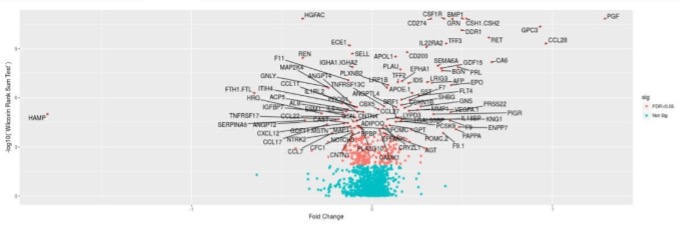
\includegraphics[width=0.7\textwidth,height=\textheight]{./step3_5.jpg}

Volcano Plot (See Below). This tab will display a scatter plot of
analytes statistical significance versus fold-change. The plot does
denote the fdr-corrected significant analytes with color coding.
Although not called out, the Fold Change on the x-axis is a log2 scale.

\newpage

\hypertarget{plotting}{%
\subsubsection{Plotting}\label{plotting}}

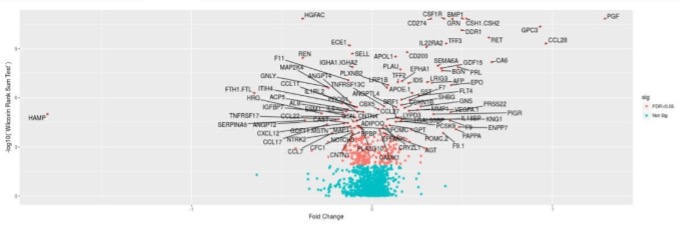
\includegraphics[width=0.7\textwidth,height=\textheight]{./step3_5.jpg}

This tool allows you to analyze individuals across any variation of
parameters on the X-Axis.\\
When analyzing data with multiple time points for each patient, you may
opt to select Join Data Points to see the connection between samples
from the same patient across data points. To use this tool, be sure the
option selected under Color matches what links your samples. For
example, if your samples were time points from the same patient and the
patient IDs are listed in the Subject column, be sure the option
selected under Color is Subject.

\newpage

\hypertarget{correlation}{%
\subsubsection{Correlation}\label{correlation}}

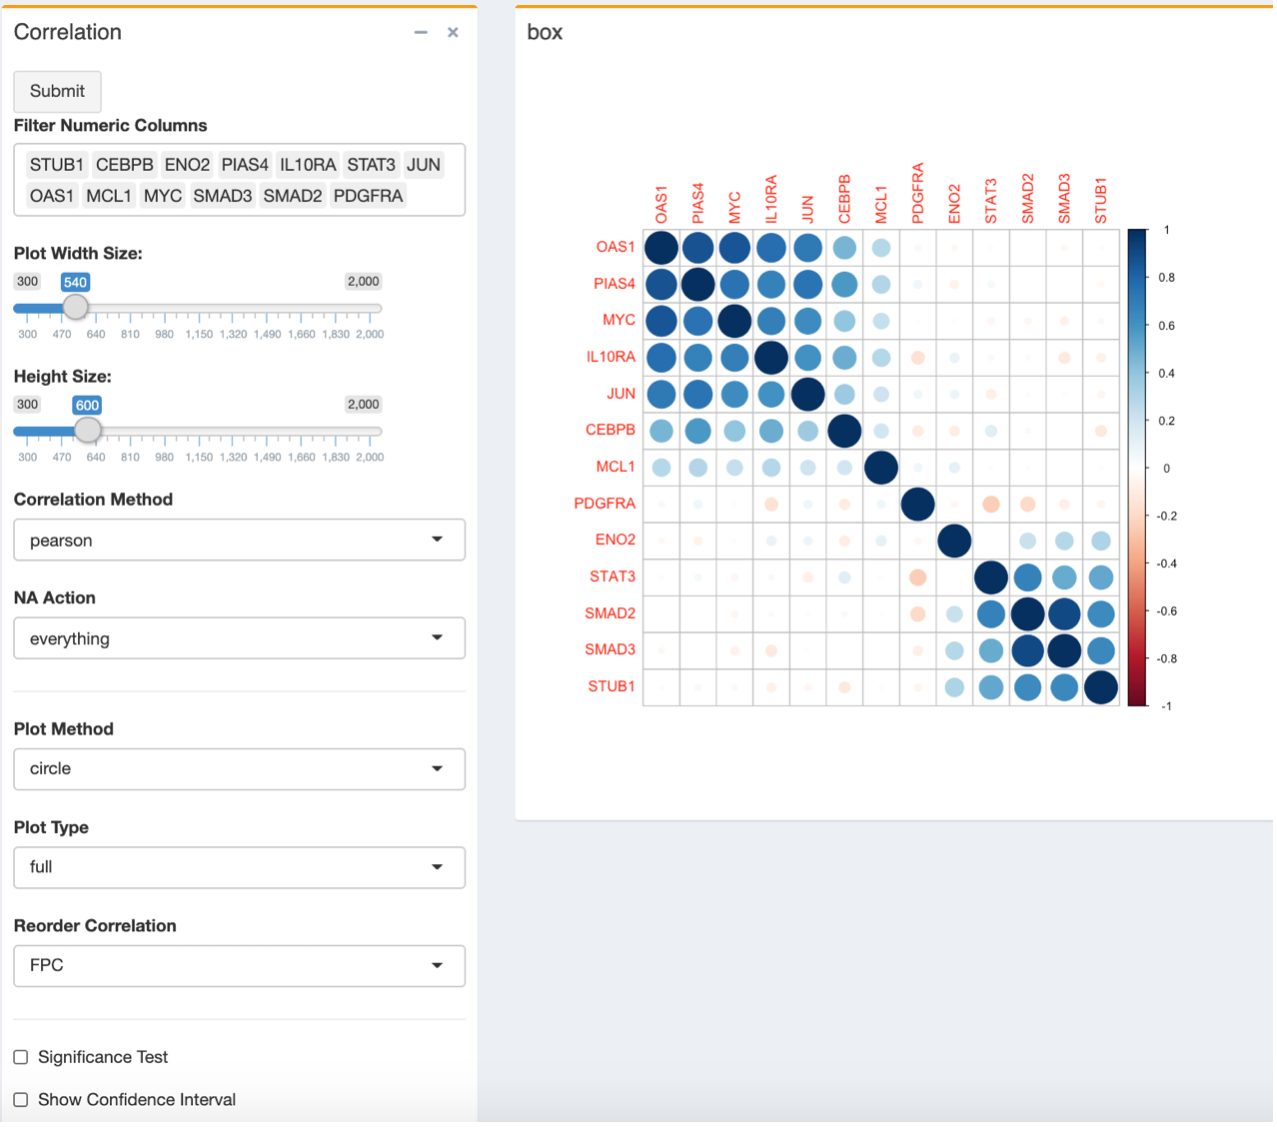
\includegraphics[width=0.7\textwidth,height=\textheight]{./step3_7.png}

We used shiny as a wrapper for the package corrplot in the Correlation
graphical display of a correlation matrix, confidence interval. It also
contains some algorithms to do matrix reordering. See documentation for
the corrplot for further details:
\url{https://CRAN.R-project.org/package=corrplot}

\newpage

\hypertarget{heatmaps}{%
\subsubsection{HeatMaps}\label{heatmaps}}

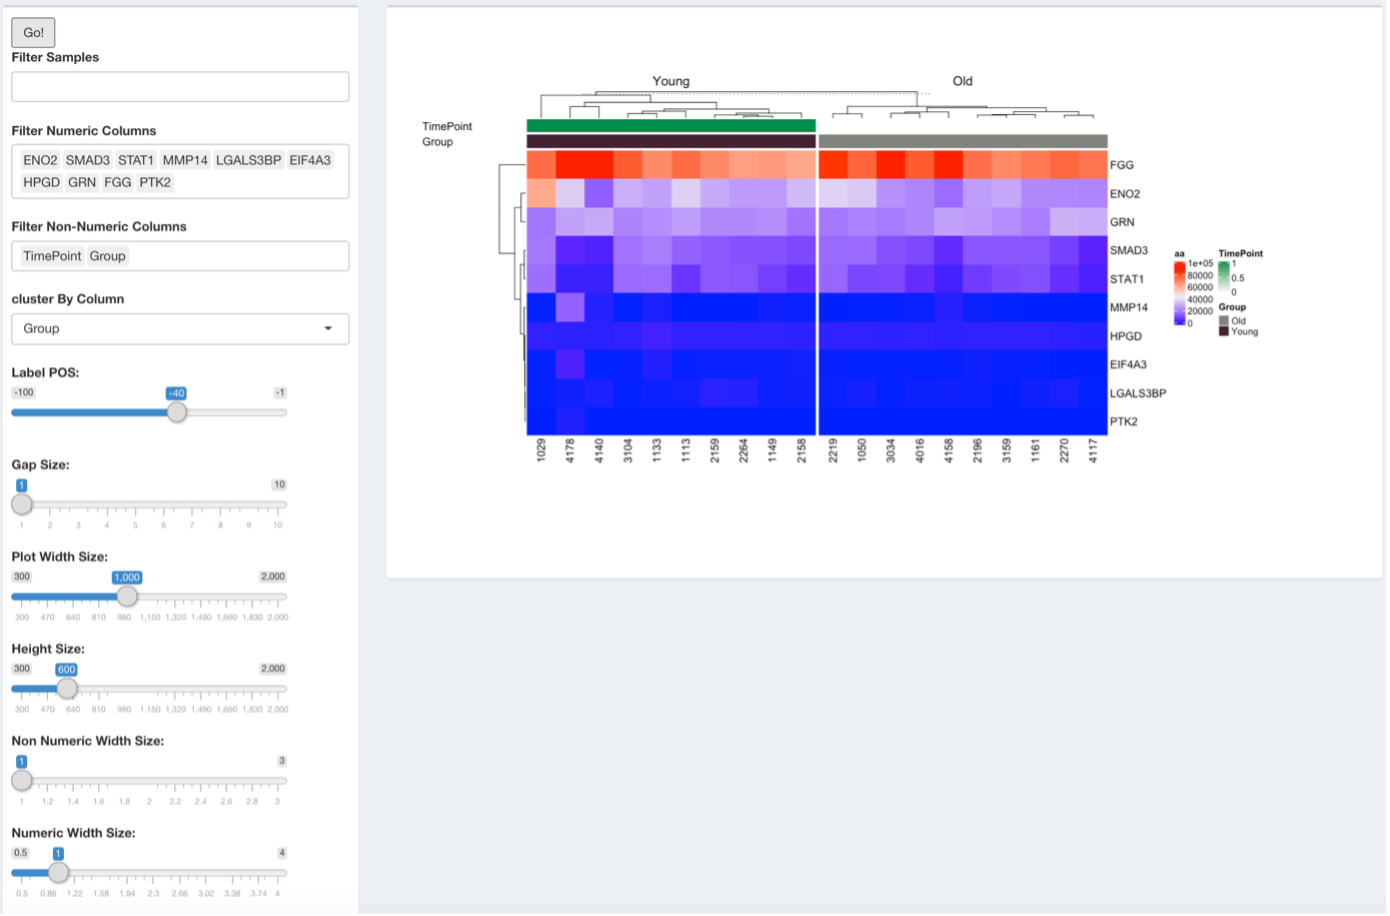
\includegraphics[width=0.7\textwidth,height=\textheight]{./step3_8.png}

We used shiny as a wrapper for some of the functions from the R package
ComplexHeatmap in the Heatmap graphical display of a matrix. See
documentation for the ComplexHeatmap for further details:
\url{https://www.bioconductor.org/packages/release/bioc/html/ComplexHeatmap.html}

\newpage

\hypertarget{coherent-chnages}{%
\subsubsection{Coherent Chnages}\label{coherent-chnages}}

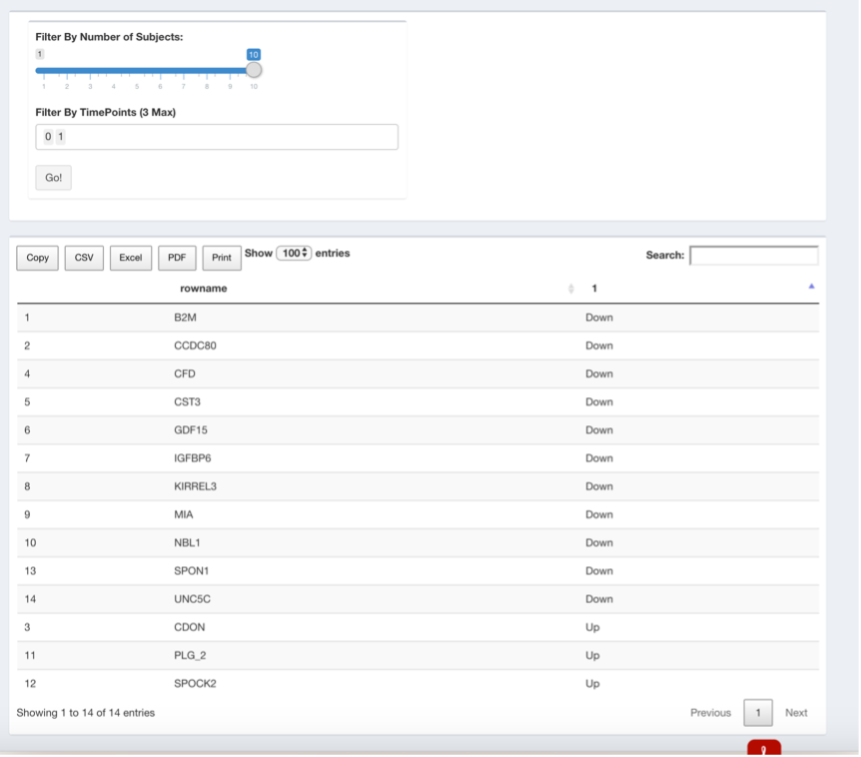
\includegraphics[width=0.7\textwidth,height=\textheight]{./step3_9.png}

This tool is valuable in identifying subjects/samples that go up or down
at each TimePoint. For example, the user may wish to know which
direction the majority of samples are going at each TimePoint. The exact
number of subjects that be determined using the select input box.

\end{document}
